% --------------------------------------------------------------------------- %
\subsection{Состояния данных}
% --------------------------------------------------------------------------- %
\begin{frame}
	\begin{figure}
		\centering
		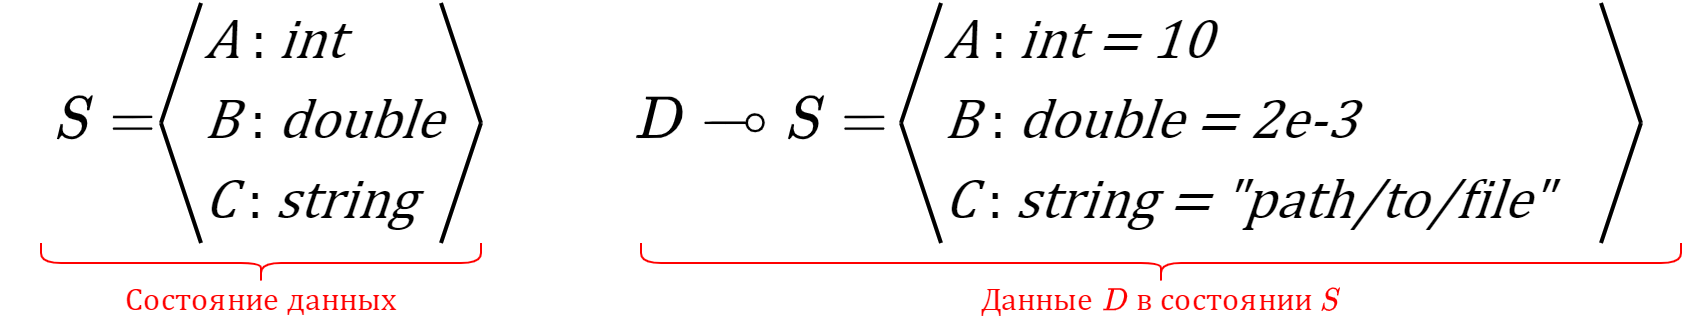
\includegraphics[width=\textwidth]{images/illustration.datastate.png}
	\end{figure}
	Состояние данных определяет, какие переменные какого типа должны быть определены на данном этапе алгоритма.

	Данные алгоритма модифицируются по ходу его выполнения.
\end{frame}

% --------------------------------------------------------------------------- %
\subsection{Функции-обработчики}
% --------------------------------------------------------------------------- %
\begin{frame}
	\begin{figure}
		\centering
		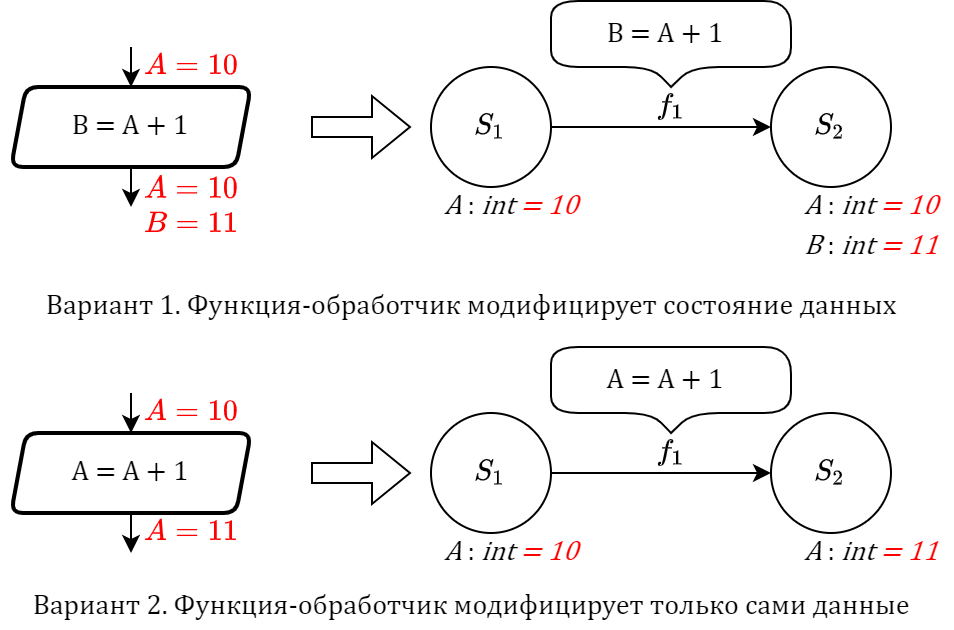
\includegraphics[width=0.7\textwidth]{images/illustration.transfer.png}
	\end{figure}

	Функции-обработчики отвечают за обработку данных и их перевод из одного состояния в другое.
\end{frame}


% --------------------------------------------------------------------------- %
\subsection{Функции-предикаты и функции перехода}
% --------------------------------------------------------------------------- %
\begin{frame}
	\begin{figure}
		\begin{minipage}{0.49\textwidth}
			\centering
			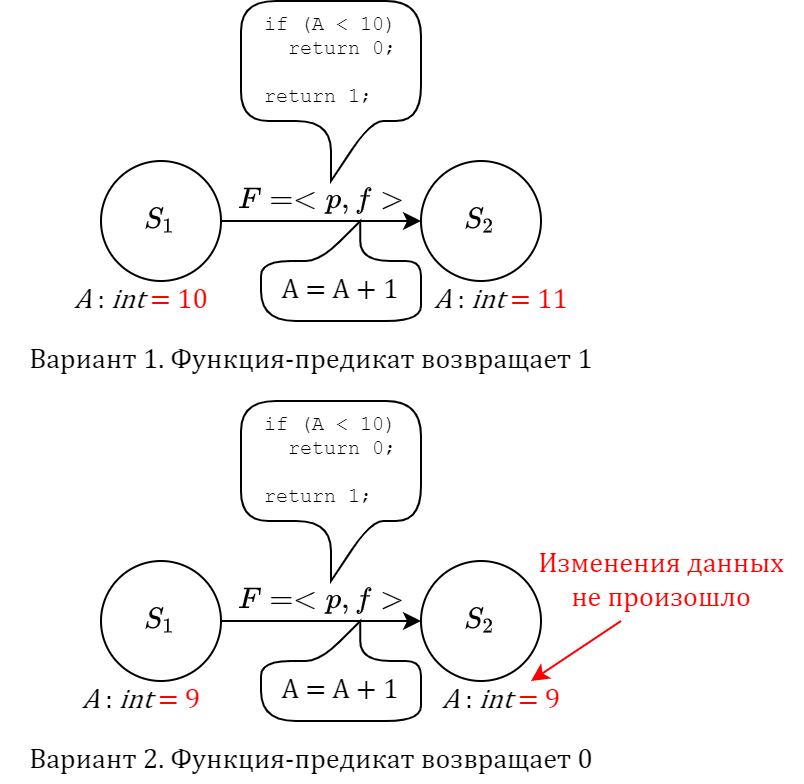
\includegraphics[height=0.5\textheight]{images/illustration.predicate.png}
			\caption{Принцип работы функции-предиката}
		\end{minipage}\hfill\begin{minipage}{0.49\textwidth}
			\centering
			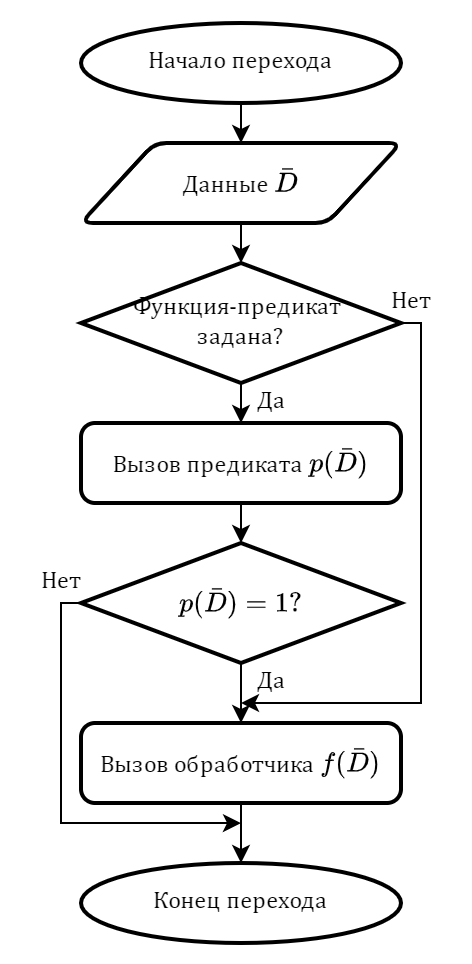
\includegraphics[height=0.5\textheight]{images/flowchart.Transfer.png}
			\caption{Блок-схема логики функции перехода}
		\end{minipage}\hfill
	\end{figure}

	Функции-предикаты отвечают за предварительную проверку данных перед их обработкой.

	Функция перехода -- составная функция $F=<p,f>$, содержащая в себе функцию-предикат $p$ и функцию-обработчик $f$.
\end{frame}

% --------------------------------------------------------------------------- %
\subsection{Функции-селекторы}
% --------------------------------------------------------------------------- %

\begin{frame}
	Функции-селекторы отвечают за проверку условий при ветвлении алгоритма.

	\begin{figure}
		\centering
		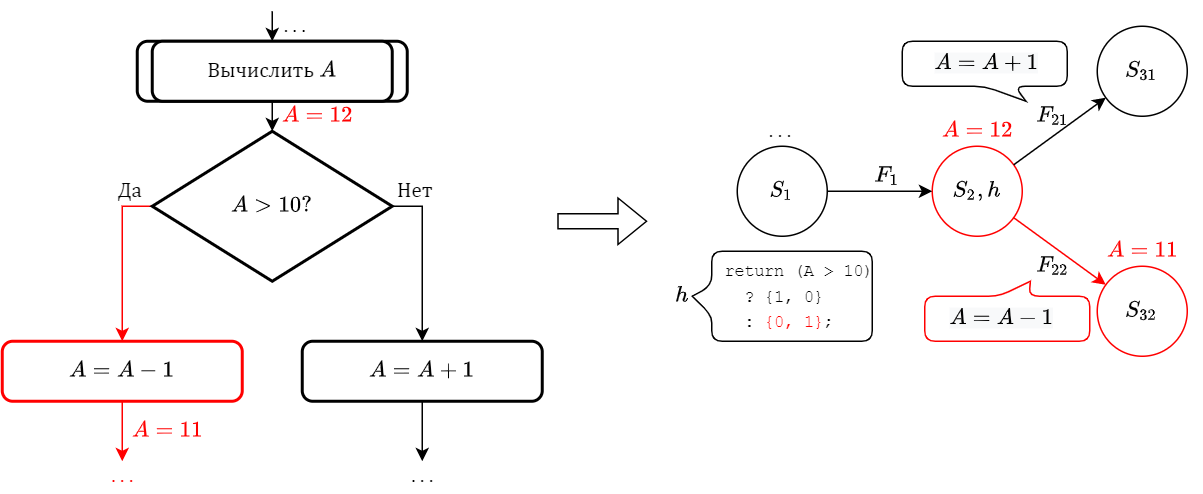
\includegraphics[width=0.9\textwidth]{images/illustration.selector.png}
		\caption{Принцип работы функций-селекторов. $h$ -- функция селектор. Красным показана ветвь алгоритма, которая будет выполнена.}
	\end{figure}
\end{frame}

% --------------------------------------------------------------------------- %
\subsection{Графовая модель}
% --------------------------------------------------------------------------- %
\begin{frame}
	Графовая модель сложного вычислительного метода описывает его логику в виде ориентированного графа, где узлам ставятся в соответствие состояния данных, а рёбрам -- функции перехода.

	\begin{figure}
		\centering
		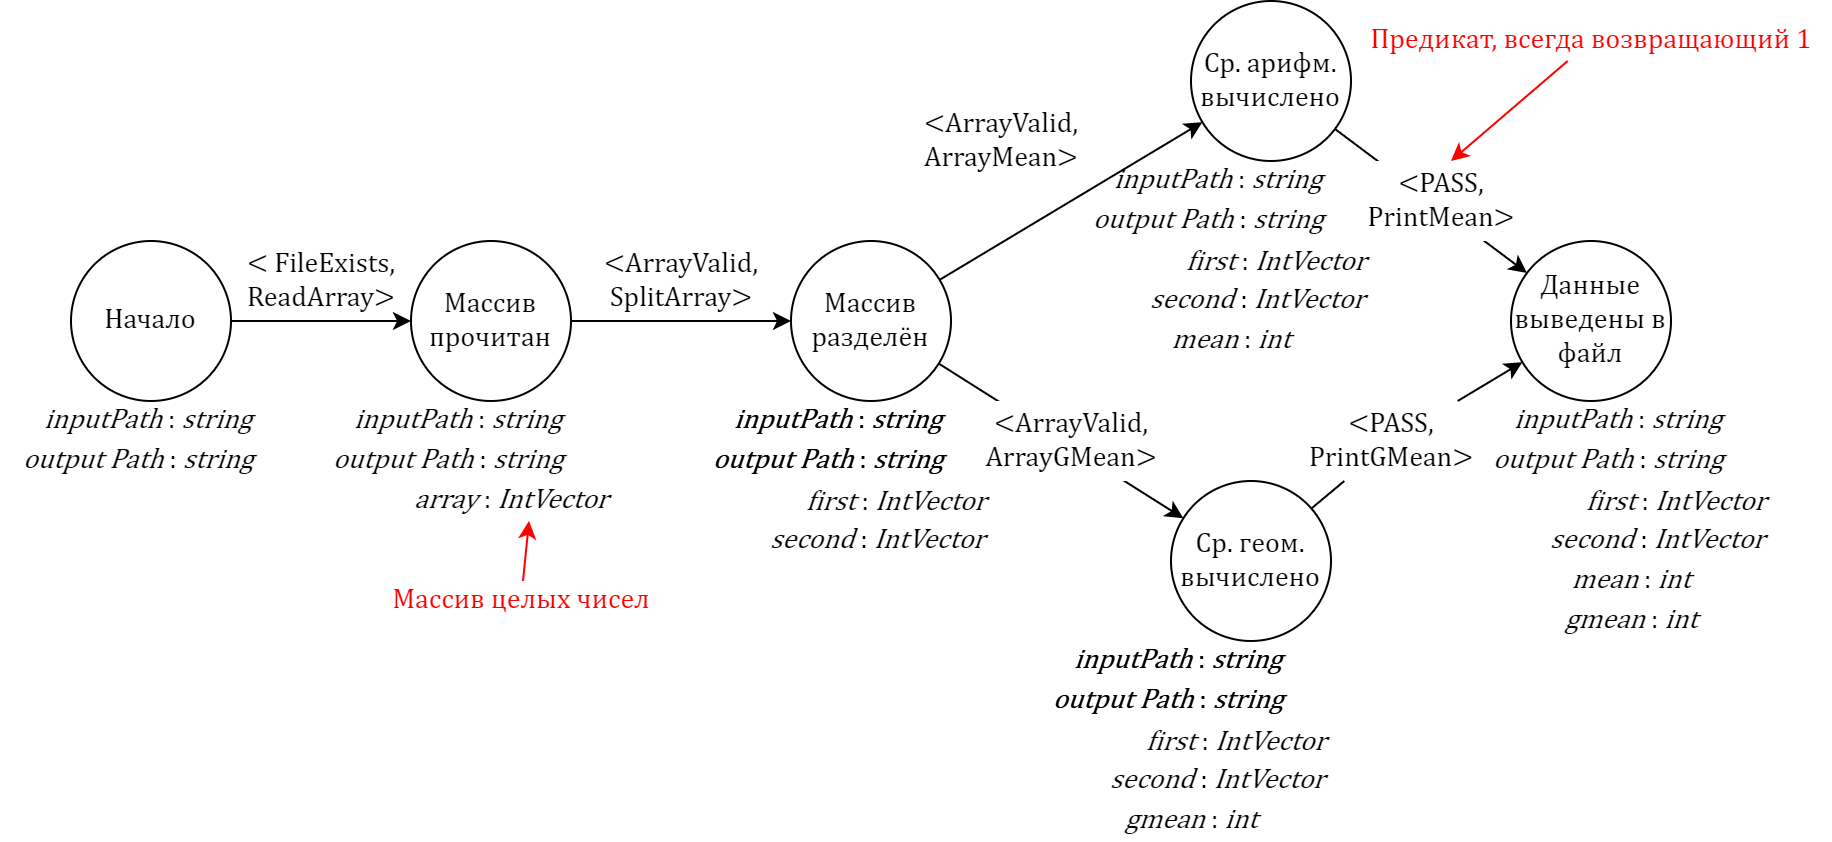
\includegraphics[width=\textwidth]{images/illustration.graph.png}
		\caption{Пример графовой модели, описывающей вычисление среднего арифметического и среднего геометрического двух половин массива целых чисел с последующей записью результатов в файл}
	\end{figure}

\end{frame}

\begin{frame}
	\begin{figure}
		\begin{minipage}{0.49\textwidth}
			\centering
			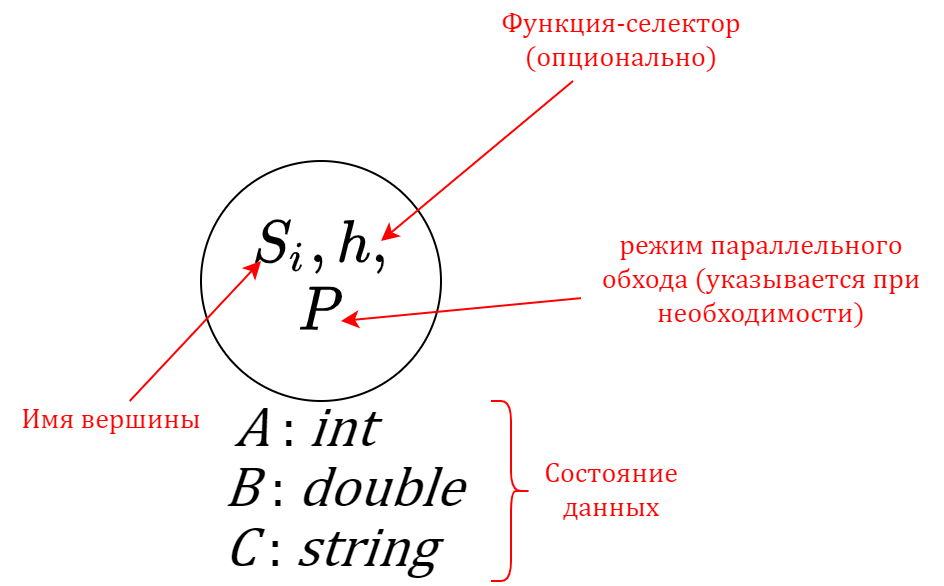
\includegraphics[width=\textwidth]{images/illustration.node.png}
		\end{minipage}\hfill\begin{minipage}{0.49\textwidth}
			Атрибуты вершины:
			\begin{enumerate}
				\item имя;
				\item состояние данных;
				\item селектор;
				\item режим параллельного обхода исходяших ветвей
			\end{enumerate}
		\end{minipage}\hfill
	\end{figure}
\end{frame}
